\documentclass[10pt, oneside]{article}
\usepackage{amsmath}
\usepackage{amssymb}
\usepackage[utf8]{inputenc}
\usepackage[english]{babel}
\usepackage{titling}
\usepackage[nottoc, notlof]{tocbibind}
\usepackage[pdftex]{graphicx}
\usepackage[kerning,spacing]{microtype}
\usepackage{verbatim}
\usepackage{tikz}
\usetikzlibrary{arrows}

\usepackage[bookmarksnumbered, unicode, pdftex]{hyperref}

\author{Mikhail Glushenkov, \texttt{<c05mgv@cs.umu.se>}\\
        Bertil Nilsson, \texttt{<id09bnn@cs.umu.se>}}

\title{Assignment 2 -- GCom Middleware:\\Final Report}

\newcommand{\unit}[1]{\ensuremath{\, \mathrm{#1}}}

\begin{document}
\pagestyle{plain}
\pdfbookmark[1]{Front page}{beg}

\begin{titlingpage}
  \begin{minipage}[t]{0.45\textwidth}
  \begin{flushleft}
  \texttt{5DV020 - Distributed Systems, Autumn 12}
  \end{flushleft}
  \end{minipage}
  \begin{minipage}[t]{0.4\textwidth}
  \begin{flushright}
  \texttt{Umeå University}
  \end{flushright}
  \end{minipage}
  \vskip 60pt
  \begin{center}
  \LARGE\thetitle
  \par\end{center}\vskip 0.5em
  \begin{center}
  \large\theauthor
  \par\end{center}
  \begin{center}
  Date: \today
  \par\end{center}
  \vfill
  \begin{center}
    \textbf{Instructors} \linebreak \linebreak
    Francisco Hernandez-Rodriguez\\
    Ewnetu Bayuh Lakew
  \end{center}
\end{titlingpage}

% TOC
%\thispagestyle{empty}
%\pagebreak
%\setcounter{page}{0}
%\pdfbookmark[1]{Table of contents}{tab}
%\tableofcontents
\pagebreak

% % i Sverige har vi normalt inget indrag vid nytt stycke
\setlength{\parindent}{0pt}
% men däremot lite mellanrum
\setlength{\parskip}{10pt}

\setcounter{section}{-1}

\section{Introduction}

The purpose of this assignment was to design and implement GCom, a middleware for
group communication. Middleware is a software layer that provides a high-level
interface to some functionality and frees the user from worrying about how said
functionality is implemented. Group communication is a mode of communication
that allows a set of nodes distributed over network to form groups and broadcast
messages to all members of the groups they belong to.

This is the final report, written at the completion stage.

\section{User's Guide}

The executable files can be found on the department's computer systems, in the
directory \texttt{/c/c05/c05mgv/5dv020}. The source code for the assignment can
be found on GitHub under the address
\texttt{https://github.com/23Skidoo/5dv020}.

To run the name server, use the following command:
\begin{center}\texttt{gcom-nameserver [-p PORT]}\end{center}
The name server expects an RMI registry to be running on local host on the port
\texttt{PORT}.

To run the combined test/debugging application, use the following command:
\begin{center}\texttt{gcom-client -p PORT -c RELIABILITY -o ORDERING  -n
    NAMESERVER -l NUMNODES COMMAND}\end{center}
Here, \texttt{NAMESERVER} is the address of the name server in the form of a
\texttt{name:host:port} triple, and the \texttt{COMMAND} parameter is one of
\texttt{list}, \texttt{kill NAME} or \texttt{join NAME}. The first command lists
the available groups, the second sends a ``kill'' message to the given group,
and the third joins a given group and starts the graphical interface. The
\texttt{-c} option sets the reliability mode (one of \texttt{\{reliable,
  unreliable\}}), and the \texttt{-o} option sets the ordering mode (one of
\texttt{\{unordered, fifo, causal, total, causaltotal\}}). The \texttt{-l}
option is for creating static groups -- it specifies how many nodes need to join
the group before communication starts; leaving \texttt{-l} out or setting it to
zero makes the group structure dynamic. The \texttt{-p} option has the same
meaning as for the name server (port number of the RMI registry).

To save the user from the hassle of having to deal with Java classpath, we also
provide our own registry executable (\texttt{gcom-registry}) that includes all
GCom classes inside its JAR.

\section{Requirements Specification}

This assignment is divided into three levels - the obligatory basic level and
two bonus levels that give additional points. Our solution implements the Level
2 specificaton (basic level + dynamic groups).

The GCom middleware consists of three logical modules: communication, message
ordering and group management. Additionally, we were required to implement a GUI
test application for showcasing the features of the GCom middleware and a GUI
debug application for demonstrating that it works correctly.

The communication module supports two operations: basic non-reliable multicast
and basic reliable multicast. The type of multicast and the message type are set
at module initialisation time, so only a single send operation is accessible at
runtime. This operation takes a set of node identifiers and a message as input,
and blocks until the message has been placed into the incoming message queues of
all of the recipients (it is synchronous in this sense). The communication
module also allows to register callbacks for acting upon a message delivered to
the current node -- this is used to pass control to the next layer of code.

The message ordering module is built on top of the communication module. It
allows to deliver messages according to several different orderings. The
following orderings are supported: non-ordered, FIFO, causal, total and
causal-total (described in more detail in the assignment specification and in
the textbook\cite{Textbook}). Again, the type of ordering is set at module
initialisation time. The same callback mechanism for passing control to the next
layer is used here.

The group management module is the client-facing part of the system implemented
on top of the previous two modules. It allows to create and remove groups, add
and remove group members, handles the monitoring of live nodes, keeps track of
changes in group membership, and allows to list the names of all existing
groups.

The test program is a simple distributed GUI chat program in which each chat
client instance is a node of the distributed system. It is combined

The debug application is implemented as a special client for the aforementioned
chat system that allows to watch the inner workings of the middleware. It has
the following features:
\begin{itemize}
\item Simulated packet loss (send a message to a part of the group).
\item Simulated packet rearrangement (send several messages in random order to
  different nodes).
\item Simulated packet delay (broadcast a message, but delay dispatching to some
  nodes).
\item Creation of a group with a chosen message ordering and multicast type.
\item Display of the internal state of the system (such as message queues).
\item Measurement of system performance.
\end{itemize}

\section{System Architecture}

We decided to implement our system in Scala and use Java RMI through Scala
interop for communication between nodes. The choice of Scala was motivated by
the desire to use a language that is more modern and convenient than Java, but
still allows to run on JVM. Java RMI was chosen because it was the default
option (recommended in the assignment specification) and we felt that other
messaging solutions that we looked at either didn't provide any benefit for our
use case (Finagle) or did all the required work for us (ZeroMQ).

\begin{figure}[h]
\centering
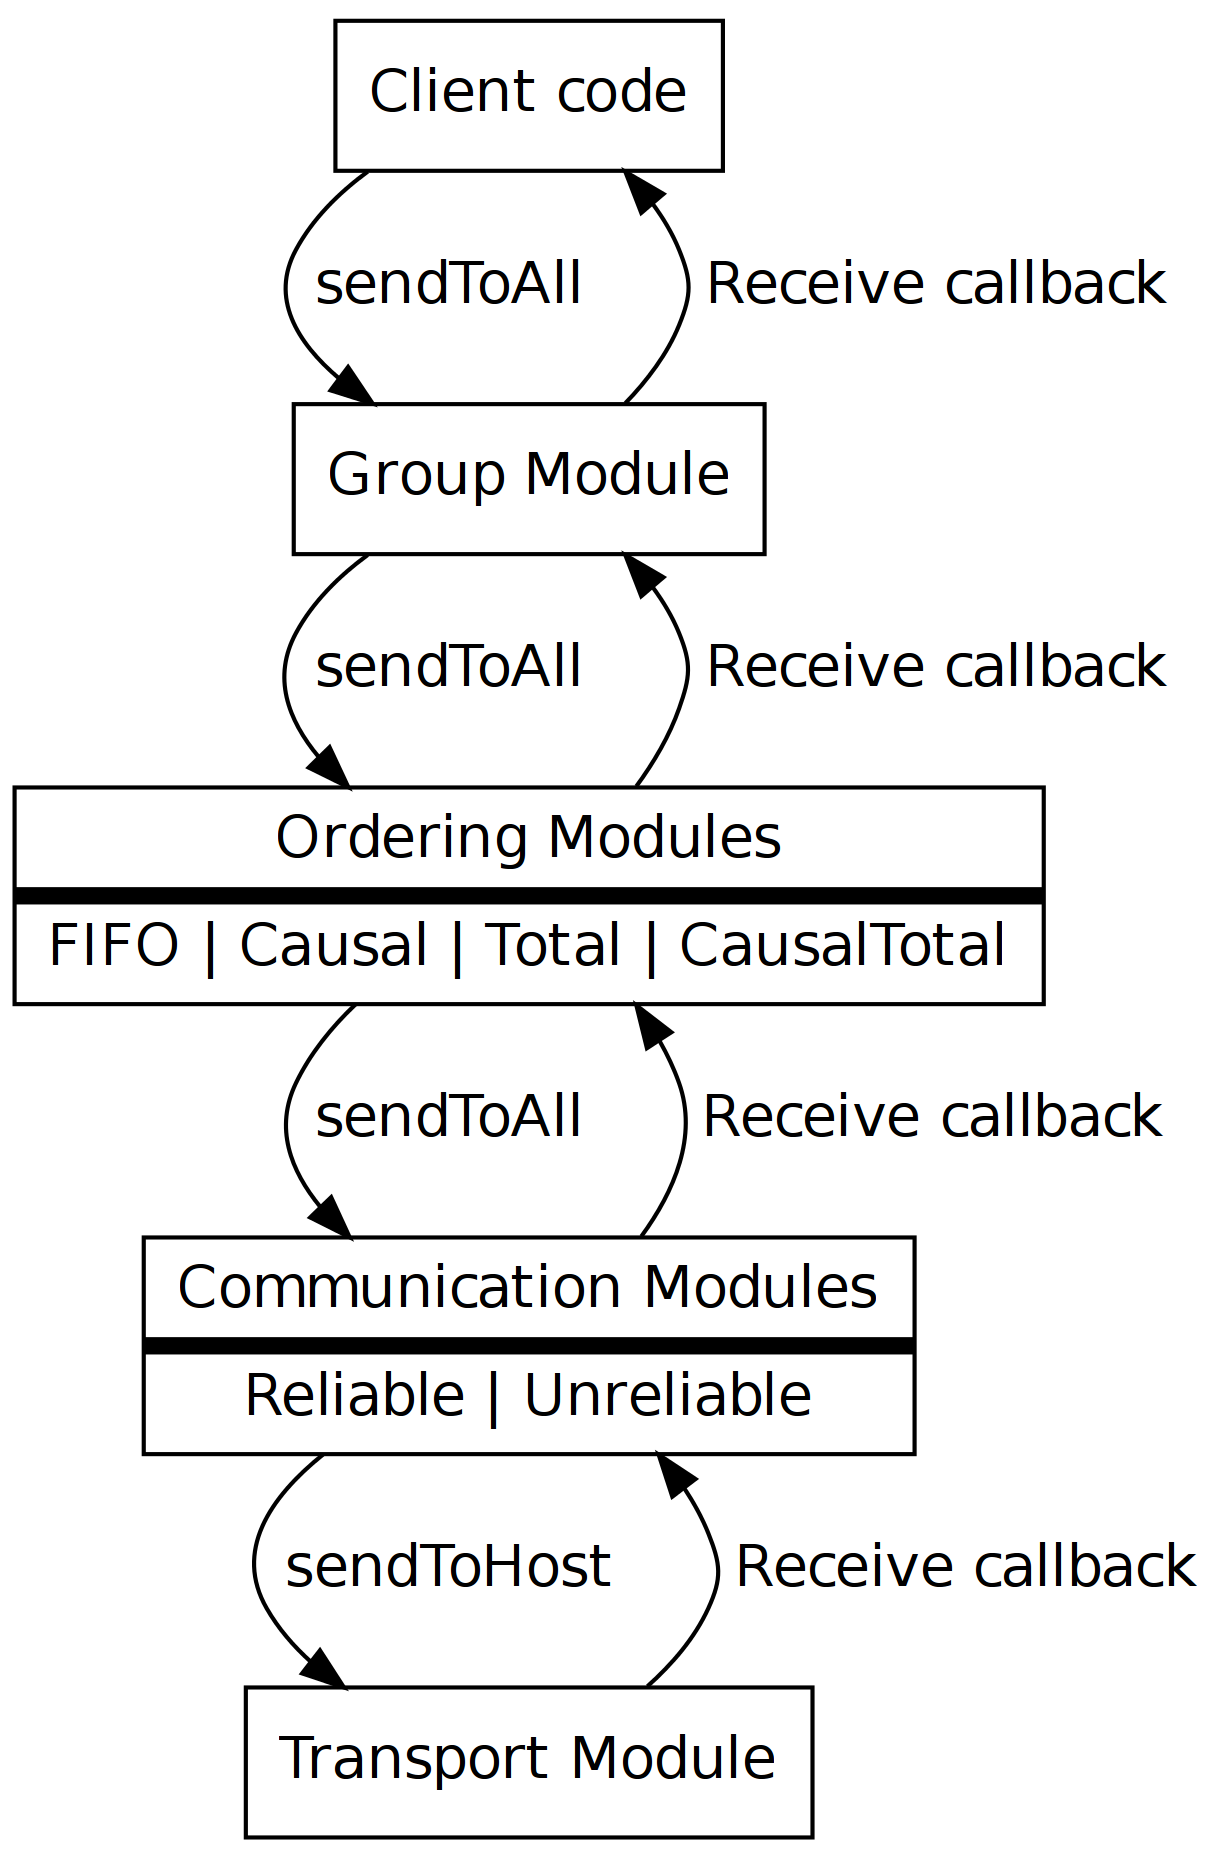
\includegraphics[height=12cm]{graph2}
\caption{Overview of the system}
\label{fig:modules}
\end{figure}

As suggested in the assignment specification, the system is decomposed into
three layers (see figure~\ref{fig:modules}):

\begin{itemize}
\item Communication
\item Message ordering
\item Group management
\end{itemize}

Each successive layer does not know anything about the layers above it - for
example, message ordering only depends on communication, but group management
uses both communication and message ordering. This improves modularity and
testability.

\subsection{Communication and message ordering}

The communication module is just a straightforward implementation of the
textbook algorithms for reliable and unreliable multicast\cite{Textbook}. The
same can be said about the message ordering module: FIFO ordering is implemented
with logical timestamps, vector clocks are used for the causal ordering, total
ordering is implemented with a sequencer node (specified as one of the inputs to
the send function), and causal-total is just a combination of causal and total.

\subsection{Group management}

\begin{figure}[h]
\centering
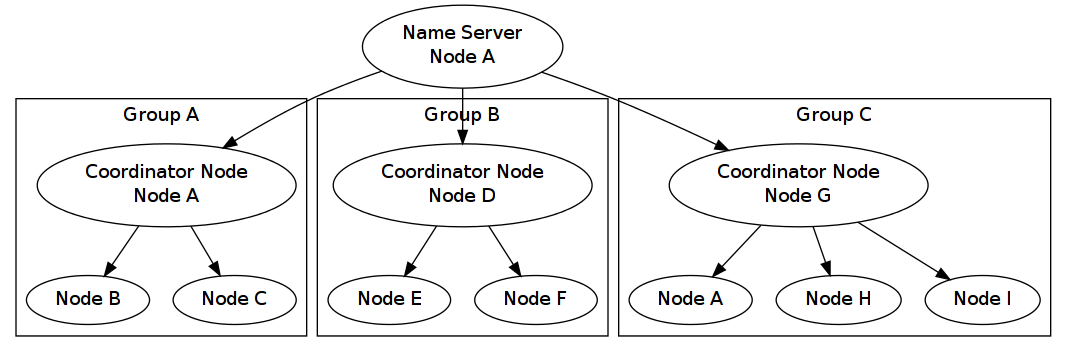
\includegraphics[width=12cm]{graph1}
\caption{Communication model used by the group management module.}
\label{fig:group}
\end{figure}

The group management module has a slightly more complicated design. Each node is
identified by a (host, port number, name) triple. A group is identified by its
name; names are globally unique, which is enforced by the name server that also
associates an ID of a coordinator node with each group name. The central server
is used as a hub through which new nodes can discover and join existing
groups. This model is illustrated in figure~\ref{fig:group}.

The coordinator node in each group serves as a gateway through which new nodes
join the group. To join a group, a node first contacts the central server, which
knows the names of all groups and all coordinator nodes. When a node has chosen
which group it wants to join, it contacts the coordinator for that group and
receives the list of all group members. The group members then synchronise its
view of group membership and the node is considered admitted.

The 2-phase commit protocol is used to ensure that all nodes have a consistent
view of group membership, group coordinator and the value of the total ordering
counter. Originally, we planned to use Paxos, but that turned out to be too
onerous to implement, and 2PC was fine for our purposes (fail-stop failure
model). Since the focus of this assignment is on multicast and message ordering,
we feel fine with a simplified solution.

The 2PC algorithm provides us with a relatively simple and straightforward way
to implement consistent shared state, which enables us to program the group
management module in a replicated state machine style (all nodes start in the
same initial state and agree on successive transitions). This simplifies
debugging and reasoning about the system.

If the coordinator node dies or leaves the group, a new coordinator is elected,
and all group members and the central server are notified. A deterministic
election algorithm is used -- the new leader is just the node with the lowest ID
number (that is, the oldest node in the group). This ensures that when two
different nodes simultaneously decide to elect a new coordinator, the same
candidate is chosen by both nodes. Thus, coordinator election can be implemented
simply as updating a single field of the shared state record, since the
immediately following updates of that field by other nodes will be idempotent.

In case a group gets partitioned, each partition will elect a new coordinator
and continue to function independently. The ones that can't contact the central
server will know that they are the ones ``left behind''. They can choose to
either shut down, continue to communicate among themselves or wait for the
central server to become available and try to rejoin the group (currently, only
the first option is implemented).

\subsection{Scalability}

The system is designed to scale fairly well, since at no point there is a need
to communicate with or store the names of all nodes in the system. Each node
communicates only with the members of the groups it belongs to, and the central
server communicates only with the coordinator nodes. The central server is
obviously a single point of failure, but the groups don't depend on it to
function and we believe that a central group catalog is needed in any case so
that new nodes can discover what groups exist in the system.

\subsection{Communication between components}

The group management module is exposed to the client, but only through the
methods defined in the Communicator interface (see
\texttt{gcom/src/GCom.scala}). On the creation of a Communicator object the
client provides the appropriate GCom settings as well as a callback to execute
when a message arrives.

Each layer in our system hooks into the lower layer by providing a callback to
call when a message is ready for the next level. To send a message the
application layer calls the \texttt{sendToAll} method of the Communicator object
which then passes the message down to lower layers. Each module adds the
specific information needed as the message passes through. This is illustrated
in figure~\ref{fig:modules}

When a layer needs to get some information from a layer above, it invokes a
callback that it was passed at creation time. For example, this is used by the
total ordering module to increment the value of the shared counter (which is
managed by the group management layer).

\subsection{Implementation of the debugger}

The graphical debugging is implemented by using the Publisher/Reactor model in
the Scala Swing wrapper. Each component extends the Publisher trait so that the
graphical user interface can listen to that component. When the components have
something new to push to the interface they publish an event containing that
specific information.

Communication in the other direction (from the interface to the GCom code --
e.g., when the user presses a button) is implemented by just calling the
appropriate methods of the corresponding GCom component from the GUI code.

\section{Limitations}

The system is designed to be scalable - we deliberately avoided algorithms that
are $O(g \times \Sigma n_g)$ in space and/or time (here, $g$ is the number of
groups and $n_g$ is the number of members in group $g$). The dependency is
either on $g$ or on $n_g$, but never on both.

The name server does not do a periodic check that group leaders are still
alive. If a whole group suddenly crashes or becomes unavailable, a stale
reference to its group leader will be preserved by the name server.

If a network gets partitioned, a partition that can't reach the name server but
includes the old leader will continue to function, while the other partition
will elect a new leader and update the name server with this information - thus,
the group will be split in two. This can be fixed by checking whether the name
server is still reachable when a group leader discovers that some nodes in the
group have become unavailable.

Messages sent out of order after a node has joined the network can be discarded
if the first message received by the node is not the first message sent. The
ordering modules will discard on individual criteria.

\pagebreak

\begin{thebibliography}{9}

\bibitem{Textbook} \emph{Distributed Systems}\\
\newblock George Coulouris, Jean Dollimore, Tim Kindberg and Gordon Blair\\
\newblock Addison-Wesley, 2011\\

\end{thebibliography}


\end{document}
